\documentclass[11pt]{amsart}
\usepackage{geometry}                % See geometry.pdf to learn the layout options. There are lots.
\geometry{letterpaper}                   % ... or a4paper or a5paper or ... 
%\geometry{landscape}                % Activate for for rotated page geometry
%\usepackage[parfill]{parskip}    % Activate to begin paragraphs with an empty line rather than an indent
\usepackage{graphicx}
\usepackage{amssymb}
\usepackage{epstopdf}
\usepackage{pgfplots}
\pgfplotsset{compat=1.18}

%\usepackage{natbib} % or \usepackage[backend=biber]{biblatex} for biblatex
%\addbibresource{Millerbib} % Use \addbibresource for biblatex
%\bibliography{Millerbib} % Use \bibliography for traditional BibTeX
%\bibliographystyle{plain} % Example style (e.g., plain, abbrv, alpha, apalike)
%\input{preamble}
\DeclareGraphicsRule{.tif}{png}{.png}{`convert #1 `dirname #1`/`basename #1 .tif`.png}

\title{Miller Professorship Report, 2024--2025}
\author{David Eisenbud}
%\date{}                                           % Activate to display a given date or no date

\begin{document}
\maketitle

\section{brief summary}
I am very grateful for the opportunity to be a Miller Professor this year. It has been a productive time, and the contacts I've made mean a lot to me, particularly with the biologists, two of  whose labs I visited. Many will continue long after the end of this happy period. The Miller spirit of interaction among scientists from different disciplines, and, particularly,  the support of postdocs, are very dear to my heart, and are things that I worked hard to increase (and to raise funds for) when I was Director of the mathematics institute.

{\bf If there is a way that I could continue to support the Miller Institute program, for example on an advisory committee or as a senior fellow or in some other capacity, I would be very happy to do so!}

My fundamental area of study is algebraic geometry: the qualitative study of geometric forms defined by polynomial equations. Examples of such forms that are familiar to every high school student are the curves in the plane that we call circle, ellipse, parabola, and hyperbola; they are called the conic sections because they can all be constructed by slicing a circular cone. These are all part of one family algebraically too, defined by equations involving only linear and quadratic terms. 
%They were intensely studied by mathematicians from the time of Euclid until the first third of the 19th century. Nowadays algebraic geometry is concerned with a far wider class of objects, often embedded in high-dimensional spaces, and this has led to wide field of applications from differential geometry and mathematical physics to artificial vision to robotic motion planning.

   Underpinning much work of this kind is the need to understand solutions of systems of linear equations of a certain kind. Again high-school students typically learn to solve two
linear equations in two unknowns, say ax+by = c and dx+ey = f, and what they learn is actually more sophisticated than what was known to mathematicians before about 1700. But the modern theory that can be used in algebraic geometry requires the solution of such equations when the coefficients a,b,c,d,e,f are themselves varying (perhaps as polynomials in further variables) and the solutions to be found are also systems of polynomials. 
%Such equations were first seriously studied by David Hilbert, the greatest mathematician of his day, around 1890, and became the center of a great deal of research starting in the 1950s. 

From the 1960s on, people began to understand the need to study situations where the coefficients and the solutions come from even more exotic domains, rings of functions on other algebraic varieties. In this context the complete resolution of one system of equations leads inevitably to an infinite sequence of further equations and solutions called in total an infinite free resolution.
%   It is in the context of these infinite free resolutions that my new observations, conjecture and theorems fall. Over the last 70 years, most of the work done in this area (and there has been a lot) has focused only on the numbers of independent solutions of each successive system of equations. Modern computational algebra and fast computers allow one to look much more deeply at the successive systems. 
 
   Using  power of modern computers my collaborators and I have seen many unexpected phenomena in this area, and proving some of these observations is where my research has been focused. The best results I have gotten are contained in two papers that have been accepted \cite{de0}, \cite{de0a}, a preprint \cite{de1}, a paper 
 that just needs to be written up \cite{de2} and another paper that is missing just a few details \cite{de3}. The gist of these papers is to give, in several different situations, and analysis of the \emph{sysygies}---the sets of solutions of these
 iterated linear equations. In these paper we describe a previously unexpected simplicity
 in some infinite free resolutions. 
 
 To be more specific: sometimes a system of linear equations can break into two systems whose solutions are independent of one another, perhaps in a way that is not immediately obvious. To take a trivial example, the system of two equations in two unknowns
 
\begin{align*}
 5x+3 &= 0\\
 2y-2&=0,
 \end{align*}
which obviously have nothing to do with one another, might be presented naturally as the system
\begin{align*}
 3x-2y+5&=0\\
x+2y +1 &= 0
 \end{align*}
(these equations are the difference and sum of the first two equations). 
In this case, untangling the second presentation into its two unrelated components is an easy
undergraduate exercise; but in the context of the equations encountered in free resolutions, 
it is much harder. A couple of years ago two graduate students (Devlin Mallory and Mahrud Sayrafi)
 came to me and asked whether
I knew of ANY algorithm, and I described one. They fearlessly plunged in and programmed it
with the result that one can now decompose fairly complex systems. It is easy to prove theoretically
that there are situations where the systems of equations in infinite free resolutions \emph{never}
decompose ``unexpectedly'', experiments showed that in other situations such decompositions
are very common.

This has led to a substantial part of my work this year, trying to understand and establish theoretical
conditions for such decompositions to occur. Papers \cite{de3}, \cite{de0a}, \cite{de2} and \cite{de1} are all 
devoted to results related to this pursuit.
 
   
In addition to my main research work, I finished a book that has been published by the American Mathematical Society \cite{de4}, and am now working on the revisions for a second book, submitted to the same publisher \cite{de5}. Both of these book projects were started about 10 years ago. I also gave a (remote) lecture at a research conference in Krakow, a lecture at the University of Utah, and a ``distinguished lecture''  at the University of Kansas. I was on the organizing committee of a semester-long program at the Fields Institute in Toronto, but because of the Miller Professorship I visited the program only for a few days.

My only other professional  activity was as member of the Boards of Directors of the Simons Foundation, a charitable foundation devoted to the support of basic research across the sciences; and of Math for America, a foundation devoted to the promotion of great K-12 teachers in math and the sciences.


\section{Abstract}
In modern geometry spaces are often studied by studying various sorts of functions defined on them. In algebraic geometry, the functions are often defined by polynomials. For example, a point in the plane can be specified by giving its coordinates $x,y$, and a typical polynomial function might be $x^2-y^3$. One way to study this function might be to graph its ``level sets'', that is, the sets of solutions to the equations $x^2-y^3 = a$, shown here for $a = 0,.1$ and .2.

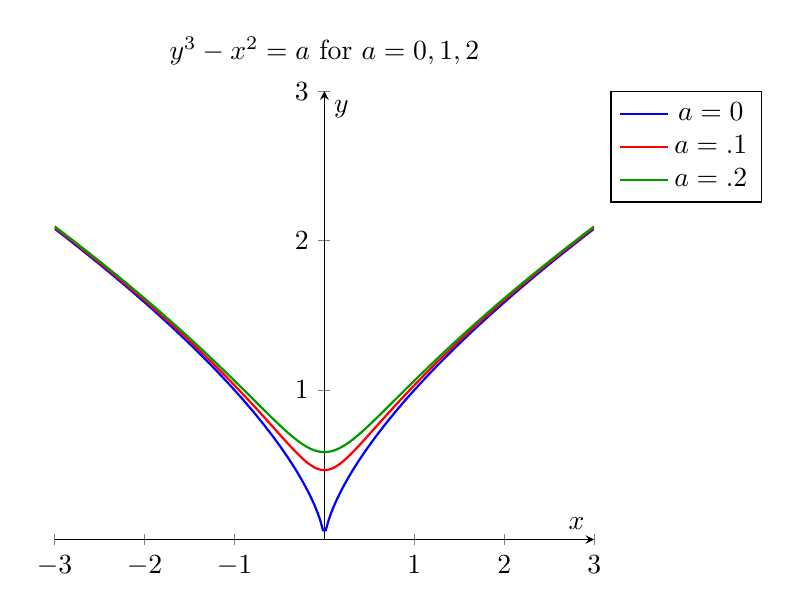
\begin{tikzpicture}
  \begin{axis}[
    axis lines = center,
    xlabel = $x$, ylabel = $y$,
    xmin=-3, xmax=3,
    ymin=0, ymax=3,
    domain=-3:3,
    samples=1000,
    legend pos=outer north east,
    title={$y^3 - x^2 = a$ for $a=0,1,2$}
  ]

    % a = 0: y^3 = x^2
    \addplot [
      domain=-3:3,
      samples=200,
      thick,
      blue
    ] ({x}, { (x^2)^(1/3) });
    \addplot [
      domain=-3:3,
      samples=200,
      thick,
      blue,
      forget plot
    ] ({x}, {- (x^2)^(1/3) });
    \addlegendentry{$a=0$}

    % a = 1: y^3 = x^2 + 1
    \addplot [
      domain=-3:3,
      samples=200,
      thick,
      red
    ] ({x}, { (x^2 + .1)^(1/3) });
    \addplot [
      domain=-3:3,
      samples=200,
      thick,
      red,
      forget plot
    ] ({x}, {- (x^2 + .1)^(1/3) });
    \addlegendentry{$a=.1$}

    % a = 2: y^3 = x^2 + 2
    \addplot [
      domain=-3:3,
      samples=200,
      thick,
      green!60!black
    ] ({x}, { (x^2 + .2)^(1/3) });
    \addplot [
      domain=-3:3,
      samples=200,
      thick,
      green!60!black,
      forget plot
    ] ({x}, {- (x^2 + 2)^(1/3) });
    \addlegendentry{$a=.2$}

  \end{axis}
\end{tikzpicture}

The blue curve is clearly special: mathematicians would say that it is \emph{singular} at the origin. My research is about the functions defined on such singular spaces in the neighborhood of a singular point.

%\subsection{}

\section{Publications}
%\nocite{*}
\bibliography{MillerReport}{}% No .bib extension needed\end{document}  
\bibliographystyle{alpha}
\end{document}
